\documentclass[letterpaper, 12pt]{article}

\setlength{\topmargin}{0in}
\setlength{\headheight}{0in}
\setlength{\headsep}{0in}
\setlength{\footskip}{0.5in}
\setlength{\textheight}{\paperheight}
\addtolength{\textheight}{-2in}
\addtolength{\textheight}{-\footskip}

\setlength{\oddsidemargin}{0in}
\setlength{\evensidemargin}{0in}
\setlength{\textwidth}{\paperwidth}
\addtolength{\textwidth}{-2in}

\pagestyle{empty}

\usepackage{amsfonts}
\usepackage{tikz}

\begin{document}

\begin{center}
\bfseries
San Jos\'{e} State University \\
Fall 2015 \\
Math-8: College Algebra \\
Section 03: MW noon--1:15pm \\
Section 05: MW 4:30--5:45pm \\
\bigskip
Quiz \#11 (Take-home)
\end{center}

\bigskip

You may use your book, notes, and homework, but please do not work together or
ask for help from others.

\bigskip

\newcommand{\fillin}{\rule{1.5in}{1pt}}

1. Consider the following graph of a polynomial function, where each grid line
represents 1 unit:

\bigskip

\begin{center}
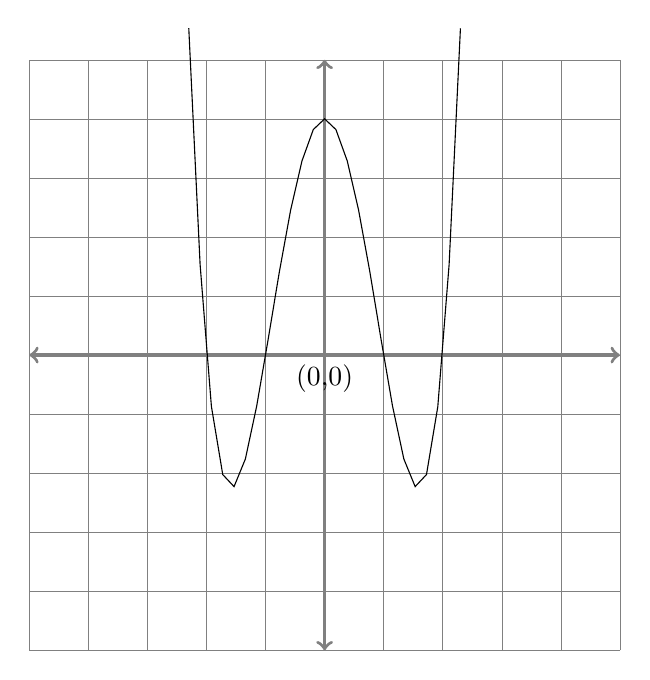
\begin{tikzpicture}[scale=0.75]
\draw [help lines] (-5,-5) grid (5,5);
\draw [help lines, <->, very thick] (-5,0) -- (5,0);
\draw [help lines, <->, very thick] (0,-5) -- (0,5);
\node [below] at (0,0) {(0,0)};
\draw [domain=-2.3:2.3] plot (\x, {(\x)^4-5*(\x)^2+4});
\end{tikzpicture}
\end{center}

\bigskip

What is the remainder when the polynomial is divided by $(x-2)$? Why?

\vspace{1in}

2. Without doing the long (or synthetic) division, what is the remainder when
$x^4-2x^3-7x^2+8x+12$ is divided by $(x+2)$? Why?

\newpage

3. Divide $x^2+1$ into $x^5-3x^2+2x-1$. Be sure to express the answer
completely.

\vspace{5in}

4. Express the answer in (4) per the division algorithm.

\newpage

5. Sketch the graph of $f(x)=x^4-2x^3-7x^2+8x+12$, showing all $x$ and $y$
intercepts, and behavior as $x\to\pm\infty$. For full credit, show how you
determined the intercepts and behavior, and how you determined the sign of
the function in between the $x$-intercepts.

\vspace{3in}

\end{document}
